\documentclass{beamer}
%\documentclass[handout]{beamer}

\usepackage{../macros}

\title{Tree}

\begin{document}

\frame{
  \titlepage
}

\begin{frame}{Tree}
  
  \begin{block}{}
    In graph theory, a tree is an \emph{undirected}, \emph{acyclic}, \emph{connected} graph
    
%    \begin{center}
%    \uncover<1->{
%    \begin{tikzpicture}
%      \node[draw, circle] (a) at (0.5, 1) {1};
%      \node[draw, circle] (b) at (1, 0) {4};
%      \node[draw, circle] (c) at (1.5, 1) {2};
%      \node[draw, circle] (d) at (0, 0) {3};
%      \node[draw, circle] (e) at (2, 0) {5};
%      
%      \draw (d) -- (a) -- (b) -- (c) -- (e);
%      
%      \uncover<2->{\draw[vert] (1, -0.25) node [below] {\ding{52}};}
%      
%      \uncover<3->{
%      \begin{scope}[xshift = 3cm]
%      \node[draw, circle] (a) at (0.5, 1) {1};
%      \node[draw, circle] (b) at (1, 0) {4};
%      \node[draw, circle] (c) at (1.5, 1) {2};
%      \node[draw, circle] (d) at (0, 0) {3};
%      \node[draw, circle] (e) at (2, 0) {5};
%      
%      \draw (d) -- (a) -- (b) -- (c) -- (e) (d) -- (b);
%      \uncover<4->{\draw[rose] (1, -0.25) node [below] {\ding{55}};}
%      \end{scope}}
%      
%      \uncover<5->{
%      \begin{scope}[xshift = 6cm]
%      \node[draw, circle] (a) at (0.5, 1) {1};
%      \node[draw, circle] (b) at (1, 0) {4};
%      \node[draw, circle] (c) at (1.5, 1) {2};
%      \node[draw, circle] (d) at (0, 0) {3};
%      \node[draw, circle] (e) at (2, 0) {5};
%      
%      \draw (d) -- (a) -- (b) (c) -- (e);
%      \uncover<6->{\draw[rose] (1, -0.25) node [below] {\ding{55}};}
%      \end{scope}}
%      
%      \uncover<7->{
%      \begin{scope}[xshift = 9cm]
%      \node[draw, circle] (a) at (0.5, 1) {1};
%      \node[draw, circle] (b) at (1, 0) {4};
%      \node[draw, circle] (c) at (1.5, 1) {2};
%      \node[draw, circle] (d) at (0, 0) {3};
%      \node[draw, circle] (e) at (2, 0) {5};
%      
%      \draw (d) -- (a) -- (b) -- (d) (c) -- (e);
%      \uncover<8->{\draw[rose] (1, -0.25) node [below] {\ding{55}};}
%      \end{scope}}
%    \end{tikzpicture}}
%    
%    \uncover<9->{Tree \emphr{$\Longrightarrow$} $n$ vertices, $n-1$ edges}
%    \end{center}
  \end{block}
%  
%  \uncover<10->{
%  \begin{block}{Search}
%    \begin{itemize}
%      \item Breadth-first search
%      \item Depth-first search
%      \begin{itemize}
%        \item Pre-order
%        \item In-order
%        \item Post-order
%      \end{itemize}
%    \end{itemize}
%  \end{block}}
\end{frame}

\begin{frame}[fragile]{Depth-first search}
  \framesubtitle{For binary trees}
  
  \begin{block}{}
    Three steps:
    \begin{itemize}
      \item[(L)] Visit the left sub-tree
      \item[(R)] Visit the right sub-tree
      \item[(N)] Visit the node
    \end{itemize}
  \end{block}
  
  \pause
  \begin{code}{Pre-order($v$) [NLR]}
    \begin{PseudoCode}
display $v$
Pre-order(left child of $v$)
Pre-order(right child of $v$)
    \end{PseudoCode}
  \end{code}  
\end{frame}

\begin{frame}[fragile]{Depth-first search}
  \framesubtitle{For binary trees}
  
  \begin{block}{}
    Three steps:
    \begin{itemize}
      \item[(L)] Visit the left sub-tree
      \item[(R)] Visit the right sub-tree
      \item[(N)] Visit the node
    \end{itemize}
  \end{block}
  
  \begin{code}{In-order($v$) [LNR]}
    \begin{PseudoCode}
In-order(left child of $v$)
display $v$
In-order(right child of $v$)
    \end{PseudoCode}
  \end{code}  
\end{frame}

\begin{frame}[fragile]{Depth-first search}
  \framesubtitle{For binary trees}
  
  \begin{block}{}
    Three steps:
    \begin{itemize}
      \item[(L)] Visit the left sub-tree
      \item[(R)] Visit the right sub-tree
      \item[(N)] Visit the node
    \end{itemize}
  \end{block}
  
  \begin{code}{Post-order($v$)  [LRN]}
    \begin{PseudoCode}
Post-order(left child of $v$)
Post-order(right child of $v$)
display $v$
    \end{PseudoCode}
  \end{code}  
\end{frame}

\begin{frame}{Depth-first search}

  \begin{center}
  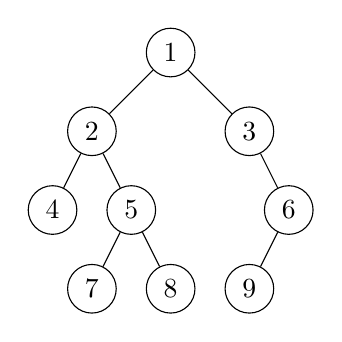
\begin{tikzpicture}
    \node[draw, circle] (1) at (1.5, 3) {1};
    \node[draw, circle] (2) at (0.5, 2) {2};
    \node[draw, circle] (3) at (2.5, 2) {3};
    \node[draw, circle] (4) at (0, 1) {4};
    \node[draw, circle] (5) at (1, 1) {5};
    \node[draw, circle] (6) at (3, 1) {6};
    \node[draw, circle] (7) at (0.5, 0) {7};
    \node[draw, circle] (8) at (1.5, 0) {8};
    \node[draw, circle] (9) at (2.5, 0) {9};
    
    \draw (1) -- (2) (1) -- (3) (2) -- (4) (2) -- (5) (3) -- (6) (5) -- (7) (5) -- (8) (6) -- (9);
    
%    \only<2-19, 31-38, 56-57|handout:0>{\node[draw, circle, rose, very thick] () at (1.5, 3) {1};}
%    \only<3-19, 21-38, 40-57|handout:0>{\draw[rose, very thick] (1) -- (2);}
%    \only<4-19, 24-38, 49-57|handout:0>{\node[draw, circle, rose, very thick] () at (0.5, 2) {2};}
%    \only<5-19, 22-38, 41-57|handout:0>{\draw[rose, very thick] (2) -- (4);}
%    \only<6-19, 23-38, 42-57|handout:0>{\node[draw, circle, rose, very thick] () at (0, 1) {4};}
%    \only<7-19, 25-38, 43-57|handout:0>{\draw[rose, very thick] (2) -- (5);}
%    \only<8-19, 28-38, 48-57|handout:0>{\node[draw, circle, rose, very thick] () at (1, 1) {5};}
%    \only<9-19, 26-38, 44-57|handout:0>{\draw[rose, very thick] (5) -- (7);}
%    \only<10-19, 27-38, 45-57|handout:0>{\node[draw, circle, rose, very thick] () at (0.5, 0) {7};}
%    \only<11-19, 29-38, 46-57|handout:0>{\draw[rose, very thick] (5) -- (8);}
%    \only<12-19, 30-38, 47-57|handout:0>{\node[draw, circle, rose, very thick] () at (1.5, 0) {8};}
%    \only<13-19, 32-38, 50-57|handout:0>{\draw[rose, very thick] (1) -- (3);}
%    \only<14-19, 33-38, 55-57|handout:0>{\node[draw, circle, rose, very thick] () at (2.5, 2) {3};}
%    \only<15-19, 34-38, 51-57|handout:0>{\draw[rose, very thick] (3) -- (6);}
%    \only<16-19, 37-38, 54-57|handout:0>{\node[draw, circle, rose, very thick] () at (3, 1) {6};}
%    \only<17-19, 35-38, 52-57|handout:0>{\draw[rose, very thick] (6) -- (9);}
%    \only<18-19, 36-38, 53-57|handout:0>{\node[draw, circle, rose, very thick] () at (2.5, 0) {9};}
  \end{tikzpicture}
  \end{center}
  
%  \begin{block}{}
%    \begin{description}
%      \item<1-58>[Pre-order] \only<2->{\only<2|handout:0>\emphr{1}} \only<4->{\only<4|handout:0>\emphr{2}} \only<6->{\only<6|handout:0>\emphr{4}} \only<8->{\only<8|handout:0>\emphr{5}} \only<10->{\only<10|handout:0>\emphr{7}} \only<12->{\only<12|handout:0>\emphr{8}} \only<14->{\only<14|handout:0>\emphr{3}} \only<16->{\only<16|handout:0>\emphr{6}} \only<18->{\only<18|handout:0>\emphr{9}}
%      \item<20->[In-order] \only<23->{\only<23|handout:0>\emphr{4}} \only<24->{\only<24|handout:0>\emphr{2}} \only<27->{\only<27|handout:0>\emphr{7}} \only<28->{\only<28|handout:0>\emphr{5}} \only<30->{\only<30|handout:0>\emphr{8}} \only<31->{\only<31|handout:0>\emphr{1}} \only<33->{\only<33|handout:0>\emphr{3}} \only<36->{\only<36|handout:0>\emphr{9}} \only<37->{\only<37|handout:0>\emphr{6}}
%      \item<39->[Post-order] \only<42->{\only<42|handout:0>\emphr{4}} \only<45->{\only<45|handout:0>\emphr{7}} \only<47->{\only<47|handout:0>\emphr{8}} \only<48->{\only<48|handout:0>\emphr{5}} \only<49->{\only<49|handout:0>\emphr{2}} \only<53->{\only<53|handout:0>\emphr{9}} \only<54->{\only<54|handout:0>\emphr{6}} \only<55->{\only<55|handout:0>\emphr{3}} \only<56->{\only<56|handout:0>\emphr{1}}
%    \end{description}
%  \end{block}
\end{frame}

\begin{frame}{Depth-first search}
%  \framesubtitle{From traversals to tree}
  \begin{overlayarea}{\textwidth}{\textheight}
  \vspace{-12pt}
  \begin{block}{Given two traversals can a tree be retrieved?}
%    \begin{itemize}
%      \item<2-> Pre-order and In-order \uncover<34-|handout:1->{\emphv{\ding{52}}}
%      \item<35-> Post-order and In-order \uncover<36-|handout:2->{\emphv{\ding{52}}}
%      \item<37-> Pre-order and Post-order \uncover<65-|handout:3->{\emphr{\ding{55}}}
%    \end{itemize}
  \end{block}
  
  \vspace{-7pt}
  
%  \only<3-34|handout:1>{
%  \begin{block}{}
%    \centering
%    \begin{tikzpicture}[scale = 0.9]
%      \draw[bleu] (0, 4.5) node[left] {Pre-order};
%      \draw[bleu] (0, 4) node[left] {In-order};
%      
%      \draw (0.25, 4.5) node {\only<4-7, 34|handout:1>\emphr{1}};
%      \draw (0.60, 4.5) node {\only<9-11|handout:0>\emphr{2}};
%      \draw (0.95, 4.5) node {\only<13-14|handout:0>\emphr{4}};
%      \draw (1.30, 4.5) node {\only<16-17|handout:0>\emphr{5}};
%      \draw (1.65, 4.5) node {\only<19-20|handout:0>\emphr{7}};
%      \draw (2.00, 4.5) node {\only<22-23|handout:0>\emphr{8}};
%      \draw (2.35, 4.5) node {\only<25-26|handout:0>\emphr{3}};
%      \draw (2.70, 4.5) node {\only<28-29|handout:0>\emphr{6}};
%      \draw (3.05, 4.5) node {\only<31-32|handout:0>\emphr{9}};
%      
%      \draw (0.25, 4.0) node {\only<14|handout:0>\emphr{4}};
%      \draw (0.60, 4.0) node {\only<10-11|handout:0>\emphr{2}};
%      \draw (0.95, 4.0) node {\only<20|handout:0>\emphr{7}};
%      \draw (1.30, 4.0) node {\only<17|handout:0>\emphr{5}};
%      \draw (1.65, 4.0) node {\only<23|handout:0>\emphr{8}};
%      \draw (2.00, 4.0) node {\only<6-7, 34|handout:1>\emphr{1}};
%      \draw (2.35, 4.0) node {\only<26|handout:0>\emphr{3}};
%      \draw (2.70, 4.0) node {\only<32|handout:0>\emphr{9}};
%      \draw (3.05, 4.0) node {\only<29|handout:0>\emphr{6}};
%     
%      
%      \uncover<8->{\node[draw, circle] (1) at (1.5, 3) {1};}
%      \uncover<12->{\node[draw, circle] (2) at (0.5, 2) {2};}
%      \uncover<27->{\node[draw, circle] (3) at (2.5, 2) {3};}
%      \uncover<15->{\node[draw, circle] (4) at (0, 1) {4};}
%      \uncover<18->{\node[draw, circle] (5) at (1, 1) {5};}
%      \uncover<30->{\node[draw, circle] (6) at (3, 1) {6};}
%      \uncover<21->{\node[draw, circle] (7) at (0.5, 0) {7};}
%      \uncover<24->{\node[draw, circle] (8) at (1.5, 0) {8};}
%      \uncover<33->{\node[draw, circle] (9) at (2.5, 0) {9};}
%      
%%    \draw (1) -- (2) (1) -- (3) (2) -- (4) (2) -- (5) (3) -- (6) (5) -- (7) (5) -- (8) (6) -- (9);
%
%      \uncover<8->{\draw (1) -- (2) (1) -- (3);}
%      \uncover<8-33|handout:0>{
%        \fill[white, fill opacity = 0.75] (0.1, 4.3) rectangle (0.4, 4.7);
%        \fill[white, fill opacity = 0.75] (1.85, 3.8) rectangle (2.15, 4.2);
%      }
%      \uncover<12->{\draw (2) -- (4) (2) -- (5);}
%      \uncover<12-33|handout:0>{
%        \fill[white, fill opacity = 0.75] (0.45, 4.3) rectangle (0.75, 4.7);
%        \fill[white, fill opacity = 0.75] (0.45, 3.8) rectangle (0.75, 4.2);
%      }
%      \uncover<15-33|handout:0>{
%        \fill[white, fill opacity = 0.75] (0.8, 4.3) rectangle (1.1, 4.7);
%        \fill[white, fill opacity = 0.75] (0.1, 3.8) rectangle (0.4, 4.2);
%      }
%      \uncover<18->{\draw (5) -- (7) (5) -- (8);}
%      \uncover<18-33|handout:0>{
%        \fill[white, fill opacity = 0.75] (1.15, 4.3) rectangle (1.45, 4.7);
%        \fill[white, fill opacity = 0.75] (1.15, 3.8) rectangle (1.45, 4.2);
%      }
%      \uncover<21-33|handout:0>{
%        \fill[white, fill opacity = 0.75] (1.5, 4.3) rectangle (1.8, 4.7);
%        \fill[white, fill opacity = 0.75] (0.8, 3.8) rectangle (1.1, 4.2);
%      }
%      \uncover<24-33|handout:0>{
%        \fill[white, fill opacity = 0.75] (1.85, 4.3) rectangle (2.15, 4.7);
%        \fill[white, fill opacity = 0.75] (1.5, 3.8) rectangle (1.8, 4.2);
%      }
%      \uncover<27->{\draw (3) -- (6);}
%      \uncover<27-33|handout:0>{
%        \fill[white, fill opacity = 0.75] (2.2, 4.3) rectangle (2.5, 4.7);
%        \fill[white, fill opacity = 0.75] (2.2, 3.8) rectangle (2.5, 4.2);
%      }
%      \uncover<30->{\draw (9) -- (6);}
%      \uncover<30-33|handout:0>{
%        \fill[white, fill opacity = 0.75] (2.55, 4.3) rectangle (2.85, 4.7);
%        \fill[white, fill opacity = 0.75] (2.9, 3.8) rectangle (3.2, 4.2);
%      }
%      \uncover<33|handout:0>{
%        \fill[white, fill opacity = 0.75] (2.9, 4.3) rectangle (3.2, 4.7);
%        \fill[white, fill opacity = 0.75] (2.55, 3.8) rectangle (2.85, 4.2);
%      }
%      
%      \only<5-7, 34|handout:1>{\node[draw, circle, rose, very thick] () at (1.5, 3) {1};}
%      \only<6-7|handout:0>{\draw[orange, very thick] (1) -- (2);}
%      \only<6-7|handout:0>{\draw[vert, very thick] (1) -- (3);}
%      \only<6-9, 34|handout:1>{\draw[orange, very thick] (0.1, 3.9) -- (0.1, 3.75) -- (1.8, 3.75) -- (1.8, 3.9);}
%      \only<6-25, 34|handout:1>{\draw[vert, very thick] (2.2, 3.9) -- (2.2, 3.75) -- (3.2, 3.75) -- (3.2, 3.9);}
%      \only<7-10, 34|handout:1>{\draw[orange, very thick] (0.45, 4.4) -- (0.45, 4.25) -- (2.15, 4.25) -- (2.15, 4.4);}
%      \only<7-26, 34|handout:1>{\draw[vert, very thick] (2.2, 4.4) -- (2.2, 4.25) -- (3.2, 4.25) -- (3.2, 4.4);}
%      
%      \only<9-11|handout:0>{\node[draw, circle, rose, very thick] () at (0.5, 2) {2};}
%      \only<10-11|handout:0>{\draw[bleu, very thick] (2) -- (4);}
%      \only<10-11|handout:0>{\draw[orange, very thick] (2) -- (5);}
%      \only<10-13|handout:0>{\draw[bleu, very thick] (0.1, 3.9) -- (0.1, 3.75) -- (0.4, 3.75) -- (0.4, 3.9);}
%      \only<10-16|handout:0>{\draw[orange, very thick] (0.8, 3.9) -- (0.8, 3.75) -- (1.8, 3.75) -- (1.8, 3.9);}
%      \only<11-14|handout:0>{\draw[bleu, very thick] (0.8, 4.4) -- (0.8, 4.25) -- (1.1, 4.25) -- (1.1, 4.4);}
%      \only<11-17|handout:0>{\draw[orange, very thick] (1.15, 4.4) -- (1.15, 4.25) -- (2.15, 4.25) -- (2.15, 4.4);}
%      
%      \only<13-14|handout:0>{\node[draw, circle, rose, very thick] () at (0, 1) {4};}
%      
%      \only<16-17|handout:0>{\node[draw, circle, rose, very thick] () at (1, 1) {5};}
%      \only<17|handout:0>{\draw[bleu, very thick] (5) -- (7);}
%      \only<17|handout:0>{\draw[orange, very thick] (5) -- (8);}
%      \only<17-19|handout:0>{\draw[bleu, very thick] (0.8, 3.9) -- (0.8, 3.75) -- (1.1, 3.75) -- (1.1, 3.9);}
%      \only<17-22|handout:0>{\draw[orange, very thick] (1.5, 3.9) -- (1.5, 3.75) -- (1.8, 3.75) -- (1.8, 3.9);}
%      \only<18-20|handout:0>{\draw[bleu, very thick] (1.5, 4.4) -- (1.5, 4.25) -- (1.8, 4.25) -- (1.8, 4.4);}
%      \only<18-23|handout:0>{\draw[orange, very thick] (1.85, 4.4) -- (1.85, 4.25) -- (2.15, 4.25) -- (2.15, 4.4);}
%      
%      \only<19-20|handout:0>{\node[draw, circle, rose, very thick] () at (0.5, 0) {7};}
%      \only<22-23|handout:0>{\node[draw, circle, rose, very thick] () at (1.5, 0) {8};}
%      
%      \only<25-26|handout:0>{\node[draw, circle, rose, very thick] () at (2.5, 2) {3};}
%      \only<26|handout:0>{\draw[vert, very thick] (3) -- (6);}
%      \only<26-28|handout:0>{\draw[vert, very thick] (2.55, 3.9) -- (2.55, 3.75) -- (3.2, 3.75) -- (3.2, 3.9);}
%      \only<27-29|handout:0>{\draw[vert, very thick] (2.55, 4.4) -- (2.55, 4.25) -- (3.2, 4.25) -- (3.2, 4.4);}
%      
%      \only<28-29|handout:0>{\node[draw, circle, rose, very thick] () at (3, 1) {6};}
%      \only<29|handout:0>{\draw[vert, very thick] (9) -- (6);}
%      \only<29-31|handout:0>{\draw[vert, very thick] (2.55, 3.9) -- (2.55, 3.75) -- (2.85, 3.75) -- (2.85, 3.9);}
%      \only<30-32|handout:0>{\draw[vert, very thick] (2.9, 4.4) -- (2.9, 4.25) -- (3.2, 4.25) -- (3.2, 4.4);}
%      
%      \only<31-32|handout:0>{\node[draw, circle, rose, very thick] () at (2.5, 0) {9};}
%      
%      
%      \only<34|handout:1>{\node[draw, circle, orange, very thick] () at (0.5, 2) {2};}
%      \only<34|handout:1>{\node[draw, circle, orange, very thick] () at (0, 1) {4};}
%      \only<34|handout:1>{\node[draw, circle, orange, very thick] () at (1, 1) {5};}
%      \only<34|handout:1>{\node[draw, circle, orange, very thick] () at (0.5, 0) {7};}
%      \only<34|handout:1>{\node[draw, circle, orange, very thick] () at (1.5, 0) {8};}
%      \only<34|handout:1>{\node[draw, circle, vert, very thick] () at (2.5, 2) {3};}
%      \only<34|handout:1>{\node[draw, circle, vert, very thick] () at (3, 1) {6};}
%      \only<34|handout:1>{\node[draw, circle, vert, very thick] () at (2.5, 0) {9};}
%    \end{tikzpicture}
%  \end{block}}
%  
%  \only<36|handout:2>{
%  \begin{block}{}
%    \centering
%    \begin{tikzpicture}[scale = 0.9]
%      \draw[bleu] (0, 4.5) node[left] {Post-order};
%      \draw[bleu] (0, 4) node[left] {In-order};
%      
%      \draw (0.25, 4.5) node {4};
%      \draw (0.60, 4.5) node {7};
%      \draw (0.95, 4.5) node {8};
%      \draw (1.30, 4.5) node {5};
%      \draw (1.65, 4.5) node {2};
%      \draw (2.00, 4.5) node {9};
%      \draw (2.35, 4.5) node {6};
%      \draw (2.70, 4.5) node {3};
%      \draw (3.05, 4.5) node {\emphr{1}};
%      
%      \draw (0.25, 4.0) node {4};
%      \draw (0.60, 4.0) node {2};
%      \draw (0.95, 4.0) node {7};
%      \draw (1.30, 4.0) node {5};
%      \draw (1.65, 4.0) node {8};
%      \draw (2.00, 4.0) node {\emphr{1}};
%      \draw (2.35, 4.0) node {3};
%      \draw (2.70, 4.0) node {9};
%      \draw (3.05, 4.0) node {6};
%     
%      \node[draw, circle, rose, very thick] (1) at (1.5, 3) {1};
%      \node[draw, circle, orange, very thick] (2) at (0.5, 2) {2};
%      \node[draw, circle, vert, very thick] (3) at (2.5, 2) {3};
%      \node[draw, circle, orange, very thick] (4) at (0, 1) {4};
%      \node[draw, circle, orange, very thick] (5) at (1, 1) {5};
%      \node[draw, circle, vert, very thick] (6) at (3, 1) {6};
%      \node[draw, circle, orange, very thick] (7) at (0.5, 0) {7};
%      \node[draw, circle, orange, very thick] (8) at (1.5, 0) {8};
%      \node[draw, circle, vert, very thick] (9) at (2.5, 0) {9};
%      
%      \draw[orange, very thick] (0.1, 3.9) -- (0.1, 3.75) -- (1.8, 3.75) -- (1.8, 3.9);
%      \draw[vert, very thick] (2.2, 3.9) -- (2.2, 3.75) -- (3.2, 3.75) -- (3.2, 3.9);
%      \draw[orange, very thick] (0.1, 4.4) -- (0.1, 4.25) -- (1.8, 4.25) -- (1.8, 4.4);
%      \draw[vert, very thick] (1.85, 4.4) -- (1.85, 4.25) -- (2.85, 4.25) -- (2.85, 4.4);
%      
%      \draw (1) -- (2) (1) -- (3) (2) -- (4) (2) -- (5) (3) -- (6) (5) -- (7) (5) -- (8) (6) -- (9);
%      
%    \end{tikzpicture}
%  \end{block}}
%  
%  \only<38-|handout:3>{
%  \begin{block}{}
%    \centering
%    \begin{tikzpicture}[scale = 0.9]
%      \draw[bleu] (0, 4.5) node[left] {Pre-order};
%      \draw[bleu] (0, 4) node[left] {Post-order};
%      
%      \draw (0.25, 4.5) node {\only<39-41|handout:0>\emphr{1}};
%      \draw (0.60, 4.5) node {\only<43-46|handout:0>\emphr{2}};
%      \draw (0.95, 4.5) node {\only<48-50|handout:0>\emphr{4}};
%      \draw (1.30, 4.5) node {\only<52-53|handout:0>\emphr{5}};
%      \draw (1.65, 4.5) node {\only<55-56|handout:0>\emphr{7}};
%      \draw (2.00, 4.5) node {\only<58-59|handout:0>\emphr{8}};
%      \draw (2.35, 4.5) node {\only<61-62|handout:0>\emphr{3}};
%      \draw (2.70, 4.5) node {\only<63-64|handout:3>\emphr{6}};
%      \draw (3.05, 4.5) node {9};
%      
%      \draw (0.25, 4.0) node {\only<49-50|handout:0>\emphr{4}};
%      \draw (0.60, 4.0) node {\only<56|handout:0>\emphr{7}};
%      \draw (0.95, 4.0) node {\only<59|handout:0>\emphr{8}};
%      \draw (1.30, 4.0) node {\only<53|handout:0>\emphr{5}};
%      \draw (1.65, 4.0) node {\only<44-46|handout:0>\emphr{2}};
%      \draw (2.00, 4.0) node {9};
%      \draw (2.35, 4.0) node {\only<64|handout:3>\emphr{6}};
%      \draw (2.70, 4.0) node {\only<62|handout:0>\emphr{3}};
%      \draw (3.05, 4.0) node {\only<40-41|handout:0>\emphr{1}};
%      
%      \uncover<47->{\draw (1) -- (2) (1) -- (3);}
%      \uncover<51->{\draw (2) -- (4) (2) -- (5);}
%      \uncover<57->{\draw (5) -- (7) (5) -- (8);}
%%      \uncover<60->{\draw (3) -- (6) (6) -- (9);}
%      
%      \uncover<42-|handout:3>{
%        \fill[white, fill opacity = 0.75] (0.1, 4.3) rectangle (0.4, 4.7);
%        \fill[white, fill opacity = 0.75] (2.9, 3.8) rectangle (3.2, 4.2);
%      }
%      \uncover<47-|handout:3>{
%        \fill[white, fill opacity = 0.75] (0.45, 4.3) rectangle (0.75, 4.7);
%        \fill[white, fill opacity = 0.75] (1.5, 3.8) rectangle (1.8, 4.2);
%      }
%      \uncover<51-|handout:3>{
%        \fill[white, fill opacity = 0.75] (0.8, 4.3) rectangle (1.1, 4.7);
%        \fill[white, fill opacity = 0.75] (0.1, 3.8) rectangle (0.4, 4.2);
%      }
%      \uncover<54-|handout:3>{
%        \fill[white, fill opacity = 0.75] (1.15, 4.3) rectangle (1.45, 4.7);
%        \fill[white, fill opacity = 0.75] (1.15, 3.8) rectangle (1.45, 4.2);
%      }
%      \uncover<57-|handout:3>{
%        \fill[white, fill opacity = 0.75] (1.4, 4.3) rectangle (1.8, 4.7);
%        \fill[white, fill opacity = 0.75] (0.45, 3.8) rectangle (0.75, 4.2);
%      }
%      \uncover<60-|handout:3>{
%        \fill[white, fill opacity = 0.75] (1.85, 4.3) rectangle (2.15, 4.7);
%        \fill[white, fill opacity = 0.75] (0.8, 3.8) rectangle (1.1, 4.2);
%      }
%      \uncover<63-|handout:3>{
%        \fill[white, fill opacity = 0.75] (2.2, 4.3) rectangle (2.5, 4.7);
%        \fill[white, fill opacity = 0.75] (2.55, 3.8) rectangle (2.85, 4.2);
%      }
%      
%      \only<44-48|handout:0>{\draw[orange, very thick] (0.1, 3.9) -- (0.1, 3.75) -- (1.45, 3.75) -- (1.45, 3.9);}
%      \only<44-61|handout:0>{\draw[vert, very thick] (1.85, 3.9) -- (1.85, 3.75) -- (2.85, 3.75) -- (2.85, 3.9);}
%      \only<46-50|handout:0>{\draw[orange, very thick] (0.8, 4.4) -- (0.8, 4.25) -- (2.15, 4.25) -- (2.15, 4.4);}
%      \only<46-62|handout:0>{\draw[vert, very thick] (2.2, 4.4) -- (2.2, 4.25) -- (3.2, 4.25) -- (3.2, 4.4);}
%      
%      \only<49-52|handout:0>{\draw[orange, very thick] (0.45, 3.9) -- (0.45, 3.75) -- (1.45, 3.75) -- (1.45, 3.9);}
%      \only<51-53|handout:0>{\draw[orange, very thick] (1.15, 4.4) -- (1.15, 4.25) -- (2.15, 4.25) -- (2.15, 4.4);}
%      
%      \only<53-55|handout:0>{\draw[orange, very thick] (0.45, 3.9) -- (0.45, 3.75) -- (1.1, 3.75) -- (1.1, 3.9);}
%      \only<54-56|handout:0>{\draw[orange, very thick] (1.5, 4.4) -- (1.5, 4.25) -- (2.15, 4.25) -- (2.15, 4.4);}
%      
%      \only<56-58|handout:0>{\draw[orange, very thick] (0.8, 3.9) -- (0.8, 3.75) -- (1.1, 3.75) -- (1.1, 3.9);}
%      \only<57-59|handout:0>{\draw[orange, very thick] (1.85, 4.4) -- (1.85, 4.25) -- (2.15, 4.25) -- (2.15, 4.4);}
%      
%      \only<62-63|handout:0>{\draw[vert, very thick] (1.85, 3.9) -- (1.85, 3.75) -- (2.5, 3.75) -- (2.5, 3.9);}
%      \only<63-|handout:3>{\draw[vert, very thick] (2.55, 4.4) -- (2.55, 4.25) -- (3.2, 4.25) -- (3.2, 4.4);}
%      
%      \only<64-|handout:3>{\draw[vert, very thick] (1.85, 3.9) -- (1.85, 3.75) -- (2.15, 3.75) -- (2.15, 3.9);}
%      
%      \uncover<42->{\node[draw, circle] (1) at (1.5, 3) {1};}
%      \uncover<47->{\node[draw, circle] (2) at (0.5, 2) {2};}
%      \uncover<63->{\node[draw, circle] (3) at (2.5, 2) {3};}
%      \uncover<51->{\node[draw, circle] (4) at (0, 1) {4};}
%      \uncover<54->{\node[draw, circle] (5) at (1, 1) {5};}
%%      \node[draw, circle] (6) at (3, 1) {6};
%      \uncover<57->{\node[draw, circle] (7) at (0.5, 0) {7};}
%      \uncover<60->{\node[draw, circle] (8) at (1.5, 0) {8};}
%%      \node[draw, circle] (9) at (2.5, 0) {9};
%     
%      \uncover<41|handout:0>{\node[draw, circle, rose, very thick] () at (1.5, 3) {1};}
%      
%      \uncover<45-46|handout:0>{
%        \node[draw, circle, rose, very thick] () at (0.5, 2) {2};
%        \draw[rose, very thick] (1) -- (2);
%        \draw[vert, very thick] (1) -- (3);
%      }
%      
%      \uncover<50|handout:0>{
%        \node[draw, circle, rose, very thick] () at (0, 1) {4};
%        \draw[rose, very thick] (2) -- (4);
%        \draw[orange, very thick] (2) -- (5);
%      }
%      
%      \uncover<53|handout:0>{\node[draw, circle, rose, very thick] () at (1, 1) {5};}
%      
%      \uncover<56|handout:0>{
%        \node[draw, circle, rose, very thick] () at (0.5, 0) {7};
%        \draw[rose, very thick] (5) -- (7);
%        \draw[orange, very thick] (5) -- (8);
%      }
%      
%      \uncover<59|handout:0>{\node[draw, circle, rose, very thick] () at (1.5, 0) {8};}
%      
%      \uncover<62|handout:0>{\node[draw, circle, rose, very thick] () at (2.5, 2) {3};}
%      
%      \uncover<64|handout:3>{
%        \node[draw, circle, rose, very thick, opacity = 0.5] (a) at (2, 1) {6};
%        \node[draw, circle, rose, very thick, opacity = 0.5] (b) at (3, 1) {6};
%        \draw[rose, very thick, dotted] (3) -- (a) (3) -- (b);
%      }
%      
%      
%    \end{tikzpicture}
%  \end{block}}
  \end{overlayarea}
\end{frame}

\end{document}
